
% WARN: arrivato a pagina 26 del pdf 1

\chapter{Lezione 25 Settembre 2023}

\section{L'azienda - ente}




Ogni azienda ha diversi macrotemi che ricadono in:
\begin{itemize}
  \item Profittabilità, no-profit
  \item Missione
  \item Visione
  \item Core business
  \item Organizzazione e struttura
\end{itemize}


Una separazione sulla base del profitto è:
\begin{itemize}
  \item \textbf{Azienda rivolta al profitto}
  \item \textbf{Organizzazione no-profit}
  \item \textbf{Ente pubblico}
\end{itemize}



\subsection{Missione}
Lo scopo dell'azienda, la sua dichiarazione d'intenti, questa \textit{frasetta} giustifica
l'esistenza dell'azienda e ci\`o che la distingue dalle altre.

Tendenzialmente il mission statement ricade nell'essere lo slogan aziendale,
anche se in alcuni casi è esaustivo e spiega in maniera completa la missione.


\subsection{Visione}

Indica la proiezione di uno scenario futuro che deve rispettare gli \textbf{ideali},
\textbf{valori} e \textbf{aspirazioni} dell'azienda.

La visione forma un'\textit{obiettivo di lungo periodo} che la dirigenza fissa per l'azienda.


\subsection{Core business}

Il core business è l'attività principale dell'azienza dal punto di vista operativo,
ne determina il compito fondaentale ed è ciò che porta fatturato.

Il core business è supportato da altre attività aziendali come \textbf{organizzazione},
\textbf{pianificazione}, \textbf{strategia} e \textbf{strumenti}.

\subsection{Parametri contabili fondamentali}

\begin{itemize}
  \item \textbf{Ricavi}: Entrate conseguite alla vendita di prodotti e servizi
  \item \textbf{Costi}: Spese sostenute per il funzionmento aziendale
  \item \textbf{Utili}: Differenza tra ricavi e costi
\end{itemize}


\subsection{Organizzazione e struttura}
La struttura organizzativa dell'azienda o ente segue una divisione in divisioni funzionali e gerarchiche.


La divisione funzionale divide l'ente in eparti, dipartimenti e divisioni, mentre la divisione gerarchica
divide per livelli di autorità:
\begin{enumerate}
  \item \textbf{Dirigenza centrale}: (Consiglio di amministrazione, direttore generale, direttore finanziario) Strategia globale
  \item \textbf{Dirigenza intermedia}: (Responsabile divisione, responsabile dipartimento) Tattica
  \item \textbf{Dirigenza operativa}: (Capo reparto, capo ufficio) Gestione delle operazioni
  \item \textbf{Reparti operativi}: (Impiegati, operai) Attività operative
\end{enumerate}

L'organigramma è un metodo di rappresentazione grafica della struttura organizzativa dell'ente.

Gli organigrammi prinicpali sono:
\begin{itemize}
  \item Organigramma verticale
  \item Organigramma radiale
\end{itemize}


\subsection{Legge di Martec}
La legge di \textbf{Martec} afferma che lo sviluppo tecnoogico \`e \textbf{esponenziale} 
mentre l'azienda ha un'andamento \textbf{logaritmico}.

\begin{figure}[!ht]
  \centering
  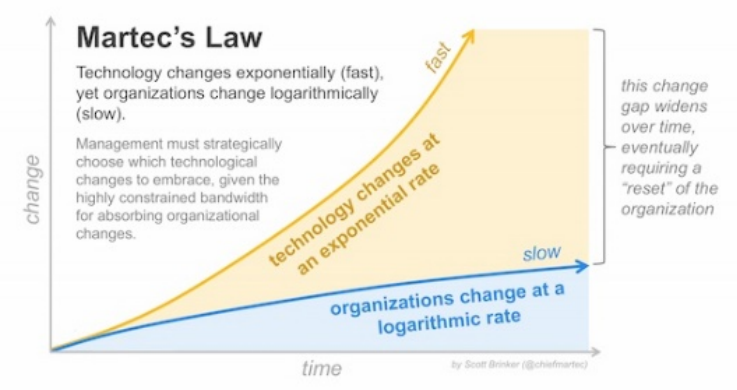
\includegraphics[width=0.7\linewidth]{images/martec.png}
  \label{fig:martec}
  \caption{Legge di Martec}
\end{figure}

Il \textit{gap} che si viene a creare tra lo sviluppo tecnologico e l'azienda necessita di un \textit{reset} da 
parte dell'azienda per poter essere colmato, solitamente necessita di grandi investimenti e ammodernamenti.

\section{Azienda - ente informatizzato}
Il sistema informativo è sempre più presente nelle aziende e negli enti.

La definizione di \textbf{Sistema informativo} è:
\begin{quote}
L’insieme di persone, apparecchiature, procedure aziendali il cui compito è quello
di produrre le informazioni che servono per operare nell’impresa e gestirla”.
(M.De Marco)
\end{quote}




I sistemi informativi sono composti di:
\begin{itemize}
  \item \textbf{Risorse umane}: organizzazione, ruoli, responsabilità
  \item \textbf{Risorse tecnologiche}: hardware, software, reti
  \item \textbf{Risorse organizzative}: procedure, regole, WORKFLOW :)
\end{itemize}

Prendendo solo il mmiglioramento tecnoogico non comporta un miglioramento generale
del sistema informativo, va considerato nel suo insieme!


